\documentclass{beamer}
%\setbeamertemplate{caption}[numbered]{\hfill\inserttitle\hfill}
%\mode<presentation> {


% The Beamer class comes with a number of default slide themes
% which change the colors and layouts of slides. Below this is a list
% of all the themes, uncomment each in turn to see what they look like.

%\usetheme{default}
%\usetheme{AnnArbor}
\usetheme{Antibes}	%good
%\usetheme{Bergen}
%\usetheme{Berkeley}
%\usetheme{Berlin}
%\usetheme{Boadilla}	%theekthak
%\usetheme{CambridgeUS}	%Laal
%\usetheme{Copenhagen}	%theekthak
%\usetheme{Darmstadt}	%jhakaas
%\usetheme{Dresden}
%\usetheme{Frankfurt}
%\usetheme{Goettingen}	%theekthak
%\usetheme{Hannover}
%\usetheme{Ilmenau}
%\usetheme{JuanLesPins}	%Jhakaas
%\usetheme{Luebeck}
%\usetheme{Madrid}	%short titles only
%\usetheme{Malmoe}
%\usetheme{Marburg}	%jhakaas
%\usetheme{Montpellier}	%super se bhi upar
%\usetheme{PaloAlto}
%\usetheme{Pittsburgh}
%\usetheme{Rochester}
%\usetheme{Singapore}
%\usetheme{Szeged}
%\usetheme{Warsaw}

% As well as themes, the Beamer class has a number of color themes
% for any slide theme. Uncomment each of these in turn to see how it
% changes the colors of your current slide theme.

%\usecolortheme{albatross}	%neela
%\usecolortheme{beaver}		%laal
%\usecolortheme{beetle}		%grey blue
\usecolortheme{crane}		%peela
%\usecolortheme{dolphin}
%\usecolortheme{dove}		%plain grey
%\usecolortheme{fly}		%full grey
%\usecolortheme{lily}
%\usecolortheme{orchid}
%\usecolortheme{rose}
%\usecolortheme{seagull}
%\usecolortheme{seahorse}
%\usecolortheme{whale}
%\usecolortheme{wolverine}

%\setbeamertemplate{footline} % To remove the footer line in all slides uncomment this line
%\setbeamertemplate{footline}[page number] % To replace the footer line in all slides with a simple slide count uncomment this line

%\setbeamertemplate{navigation symbols}{} % To remove the navigation symbols from the bottom of all slides uncomment this line
%}

\usepackage{color}
\usepackage{verbatim}

\begin{document}
\title{\textbf{Title:} Reading Aid using OCR, web search and text to speech conversion}
\author{Neeraj Babu, Sonal Gupta}
\setbeamertemplate{navigation symbols}{}
\setbeamertemplate{footline}{\parbox{\linewidth}{\vspace*{-8pt}\hfill\insertpagenumber\hfill\insertshortauthor\hfill}}
\setbeamertemplate{headline}{\parbox{\linewidth}{\vspace*{-18pt}\hspace{10pt}\small\inserttitle\hfill}}
\institute{Department of Electrical Engineering\\IIT Bombay}
\date{} 
%\frame{\titlepage}

\frame{\frametitle{Project Objective}
	\begin{itemize}
		\item Read out text from an image to facilitate reading for
			a blind person.
		\item Read out meaning of an underlined word in a text.
		\item Read out details of a word, person, place etc. through web search.
	\end{itemize}
}

\frame{\frametitle{Implementation Algorithm}
START:  Start the reader\\
        \hspace{35pt}Click photo through webcam\\
        \hspace{35pt}Extract underlined text through opencv\\
        \hspace{35pt}Option = user input\\
        \hspace{35pt}if (Option == read out)\\
        \hspace{55pt}    Read out the text\\
        \hspace{35pt}else if (Option == image)\\
        \hspace{55pt}    Show image of the underlined\\
        \hspace{55pt}    text on screen\\
}

\frame{\frametitle{Implementation Algorithm}
        \hspace{35pt}else if (Option == wiki)\\
        \hspace{55pt}    Do a wiki search of the\\
        \hspace{55pt}    underlined text\\
        \hspace{35pt}else\\
        \hspace{55pt}    Show meaning of the\\
        \hspace{55pt}    underlined text\\
        \hspace{35pt}Destroy files and images\\
        \hspace{35pt}goto START\\
}

\frame{\frametitle{Software Overview}
	\begin{figure}
		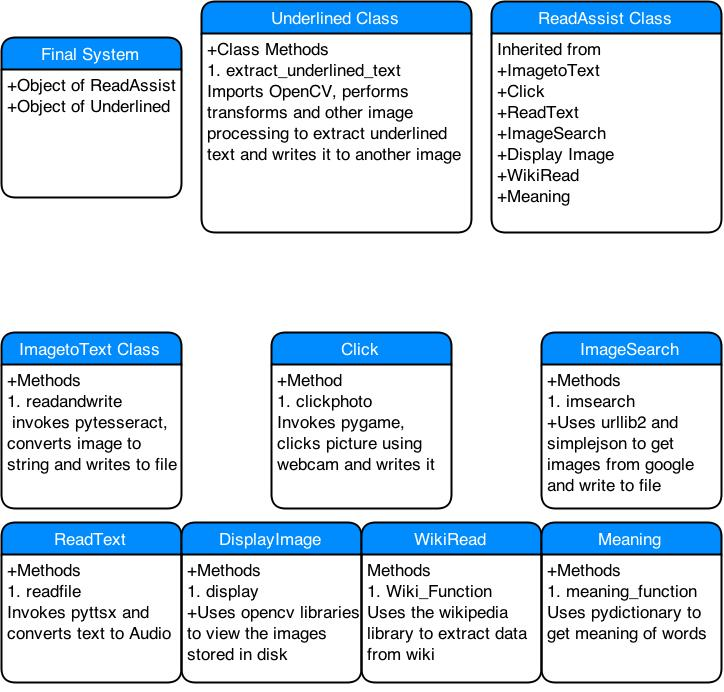
\includegraphics[width=0.65\linewidth]{Algo.jpg}
	\end{figure}

}

\frame{\frametitle{Project Outline - Tools/Packages and Technology Stack Used}
	\begin{itemize}
		\item Clicking image and converting to text:\\
			\textcolor{blue}{pygame, pytesseract}
		\item Identifying underlined text:\\
			\textcolor{blue}{opencv}
		\item Dictionary and web search:\\
			\textcolor{blue}{PyDictionary, urllib, simplejson, wikipedia}
		\item Text to speech:\\
			\textcolor{blue}{pyttsx}
	\end{itemize}
}

\section{Modules}
\frame{\frametitle{\textbf{PyGame:} Python text to speech converter}
	PyGame has been used in our project to acquire image from
	the camera. It is capable of acquiring the image from
	inbuilt webcam or usb connected camera. Following is a snippet
	of the code used.\\
	\begin{figure}
		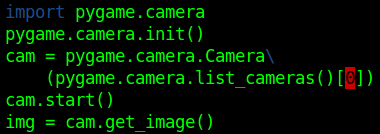
\includegraphics[width=0.55\linewidth]{images/pygame.png}
	\end{figure}
}

\frame{\frametitle{\textbf{Python-tesseract:} OCR}
	Python-tesseract is an optical character recognition 
	(OCR) tool for python. It will recognize and ``read" 
	the text embedded in images. Python-tesseract is a 
	wrapper for google's Tesseract-OCR
	The main function we used from this module is:
	\begin{figure}
		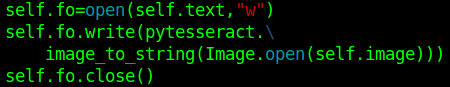
\includegraphics[width=0.55\linewidth]{images/tesseract.png}
	\end{figure}
	This method returns a text to standard output which can be written to a file.
	The image to be passed has to be sharpened to increase conversion confidence.
}

\frame{\frametitle{\textbf{OpenCV:} Image Processing IN PYTHON}
	OpenCV libraries comes in handy when we do anything 
	in image processing.  We describe some of the major 
	tasks we performed by using methods from this module.
	Following is the code used for reading image and 
	converting it to binary:
	\begin{figure}
		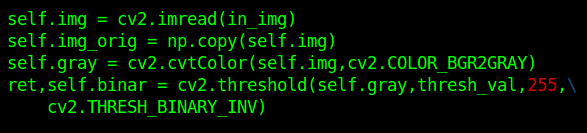
\includegraphics[width=0.75\linewidth]{images/read_image.png}
	\end{figure}
}

\frame{\frametitle{\textbf{OpenCV:} Image Processing IN PYTHON}
	Following code is used for detecting lines in the binary
	image:
	\begin{figure}
		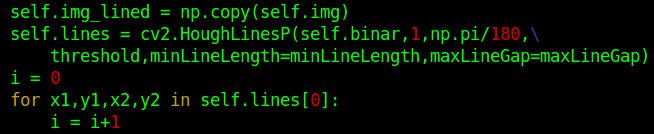
\includegraphics[width=0.75\linewidth]{images/houghlinesP.png}
	\end{figure}
	The image is then dilated to convert each word to a single
	contour:
	\begin{figure}
		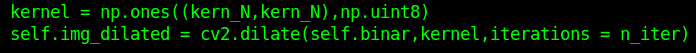
\includegraphics[width=0.75\linewidth]{images/dilate.png}
	\end{figure}
}

\frame{\frametitle{\textbf{OpenCV:} Image Processing IN PYTHON}
	Contour detection is then done on the dilated image to
	give coordinates of rectangle around each word.
	\begin{figure}
		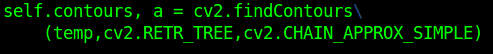
\includegraphics[width=0.75\linewidth]{images/contour.png}
	\end{figure}
	These coordinates are then compared with that of line
	obtained earlier and the underlined word is thus extracted.
}

\frame{\frametitle{\textbf{OpenCV:} Image Processing IN PYTHON}
	\begin{figure}
		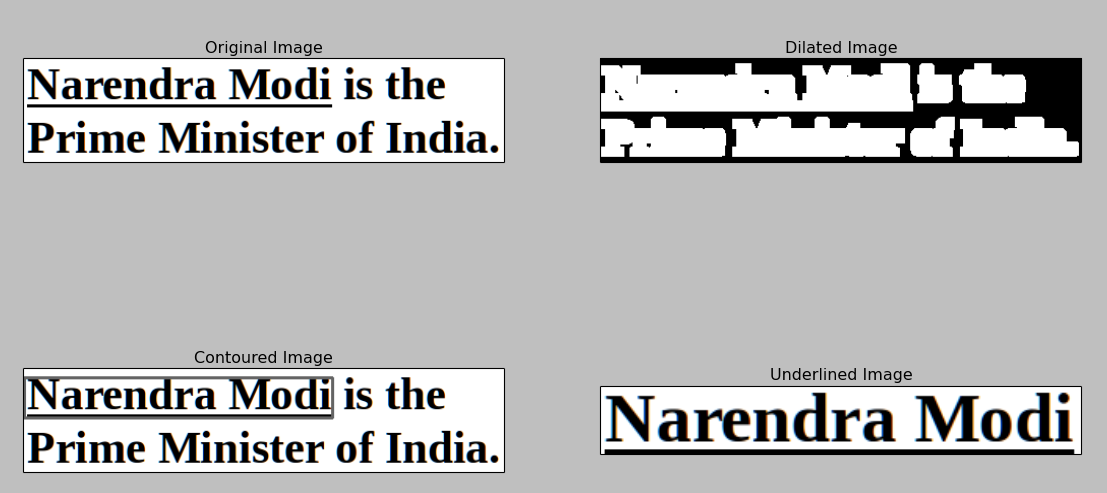
\includegraphics[width=0.85\linewidth]{images/namo.png}
	\end{figure}
}

\frame{\frametitle{\textbf{PyDictionary:} Python Dictionary Module}
	This module and it’s methods helped us in getting the 
	meanings, translations antonyms and synonyms of a word. 
	The usage is as follows:
	\begin{figure}
		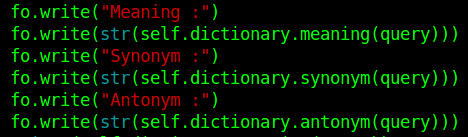
\includegraphics[width=0.75\linewidth]{images/dictionary.png}
	\end{figure}
}

\frame{\frametitle{\textbf{Urllib, Simplejson}}
	To interact with JSON, we can use the json and 
	simplejson modules in python. Once JSON object 
	is loaded into python by using the above modules, 
	it just becomes like a dictionary.\\
	An example of its use in our project 
	is to get images from google as follows:\\
	\begin{figure}
		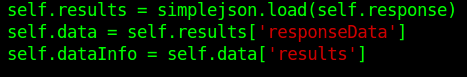
\includegraphics[width=0.75\linewidth]{images/simplejson.png}
	\end{figure}
	This gets the entire dictionary of the opened url to data. 
	From this dictionary, by applying the keys specified 
	by vendor say google, we can extract the required information.
}


\frame{\frametitle{\textbf{Pyttsx:} Python text to speech converter}
	In our application we used espeak driver for linux. 
	The init function of pyttsx creates an object of 
	\textit{pyttsx.engine.Engine} class which has the following 
	methods we used:
	\begin{itemize}
		\item \textit{setProperty()}: Sets the rate of speech and volume
		\item \textit{say(text: unicode, name: string)}: To speak out text
	\end{itemize}
	Another important class we can initialize from the module 
	is \textit{pyttsx.voice.Voice}. An object of this class 
	has methods to perform the following tasks:
	\begin{itemize}
		\item To set the language of speech
		\item To set the gender and age of the renderer
	\end{itemize}
}

\frame{\frametitle{\textbf{Results:} Google image search}
	\begin{figure}
		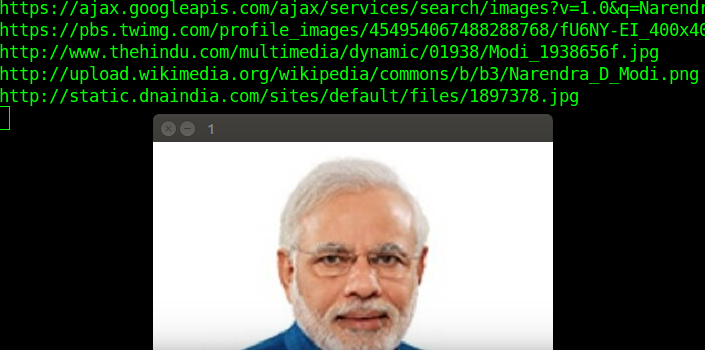
\includegraphics[width=0.85\linewidth]{images/namo_img.png}
	\end{figure}
}

\frame{\frametitle{\textbf{Results:} Wikipedia search}
	\begin{figure}
		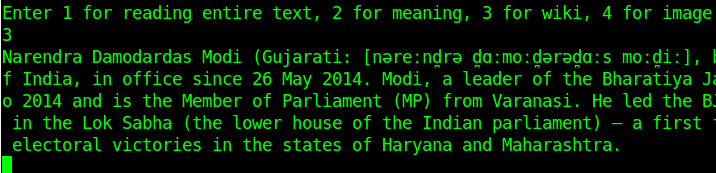
\includegraphics[width=0.85\linewidth]{images/namo_wiki.png}
	\end{figure}
}

\frame{\frametitle{\textbf{Results:} Meaning}
	\begin{figure}
		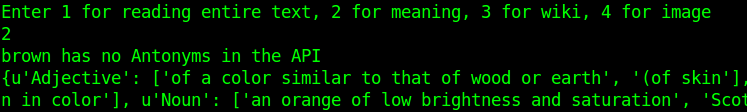
\includegraphics[width=0.85\linewidth]{images/brown_mean.png}
	\end{figure}
}

\frame{\frametitle{Thank You}
	\textbf{Repository:} \url{https://github.com/agalunstop/SDES_Readout}
}


\end{document}
